\documentclass[preprint]{elsarticle}

\usepackage{amssymb, latexsym, amsthm, amsmath,lineno,epsfig,mathtools,hyperref,todonotes,booktabs,cite}
\usepackage[singlelinecheck=false]{caption}
\modulolinenumbers[5]

\journal{Theoretical Population Biology}

%%%%%%%%%%%%%%%%%%%%%%%
%% Elsevier bibliography styles
%%%%%%%%%%%%%%%%%%%%%%%
%% To change the style, put a % in front of the second line of the current style and
%% remove the % from the second line of the style you would like to use.
%%%%%%%%%%%%%%%%%%%%%%%

%% Numbered

%\bibliographystyle{model1-num-names}

%% Numbered without titles
%\bibliographystyle{model1a-num-names}

%% Harvard
%\bibliographystyle{model2-names.bst}\biboptions{authoryear}

%% Vancouver numbered
%\usepackage{numcompress}\bibliographystyle{model3-num-names}

%% Vancouver name/year
%\usepackage{numcompress}\bibliographystyle{model4-names}\biboptions{authoryear}

%% APA style
%\bibliographystyle{model5-names}\biboptions{authoryear}

%% AMA style

%\usepackage{numcompress}\bibliographystyle{model6-num-names}

%% `Elsevier LaTeX' style
\bibliographystyle{natbibgen}
%%%%%%%%%%%%%%%%%%%%%%%

\renewcommand{\baselinestretch}{1}
\newcommand{\gdw}{\Leftrightarrow}
\newcommand{\br}{\allowdisplaybreaks}
\newcommand{\N}{\mathbb{N}}
\newcommand{\RR}{\mathbb{R}}
\newcommand{\ZZ}{\mathbb{Z}}
\newcommand{\eps}{\varepsilon}
\newcommand{\tx}{\textnormal}
\newcommand{\maxi}{\vee}
\newcommand{\mini}{\wedge}
%\newcommand{\ii}{\parallel}
\newcommand{\fett}{\textbf}
\newcommand{\T}{\textstyle}
\newcommand{\bs}[1]{\ensuremath{\boldsymbol{#1}}}

%\renewcommand{\floatpagefraction}{.8}
\newcommand\Var{\operatorname{Var}}
\newcommand\Cov{\operatorname{Cov}}
\newcommand\E{\operatorname{E}}
\newcommand\e{\operatorname{e}}
\newcommand\dbeta{\operatorname{beta}}
\newcommand\J{\operatorname{J}}
\newcommand\abs[1]{{\lvert\,#1\,\rvert}}
\newcommand\given{{\,|\,}}
\newcommand\diag[1]{{\operatorname{diag}\left(#1\right)}}
\newcommand\trps{{^{\operatorname{T}}}}
\newcommand{\norm}[1]{\left\lVert#1\right\rVert}
\newcommand\etal{{\it et~al.}}
\newcommand\eg{{\it e.g.,}}
\newcommand\cf{{\it c.f.,}}
\newcommand\ie{{\it i.e.,}}
\newcommand\bzw{{\it bzw\.}}
\newcommand\etc{{\it etc}}
\newcommand\dgr{{$^o$}}

% Dom: I decided to use X_t for time dependence instead of x(t) because it is better readable.  However, it could be redefined here, if you do not agree!
\newcommand\x[1]{\ensuremath{X_{#1}}}
% Same for y.
\newcommand\y{\ensuremath{Y}}
% Use capital or lower case letter for the time at -s?
\newcommand\s{\ensuremath{s}}
% Definitions of f, b and the one vectors.
\newcommand\fv[1]{\ensuremath{\mathbf{f}_{#1}}}
\newcommand\bv[1]{\ensuremath{\mathbf{b}_{#1}}}
\newcommand\gv[1]{\ensuremath{\mathbf{g}_{#1}}}
\newcommand\oneC{\ensuremath{\mathbf{1}'}}
\newcommand\oneR{\ensuremath{\mathbf{1}}}
% TODO: Juraj, please ignore the following line.
% CV: I associate "bs" with "bullshit"! This comment should be ignored by serious persons.

\begin{document}

\begin{frontmatter}

\title{Inference in Population Genetics Using Forward and Backward, Discrete and Continuous Time Processes}

\author[address1,address2]{Juraj Bergman}
\ead{juraj.bergman@vetmeduni.ac.at}
\author[address1,address2]{Dominik Schrempf}
\ead{juraj.bergman@vetmeduni.ac.at}
\author[address1]{Carolin Cosiol}
\ead{carolin.kosiol@vetmeduni.ac.at}
\author[address3]{Claus Vogl\corref{correspondingauthor}}
\cortext[correspondingauthor]{Corresponding author}
\ead{claus.vogl@vetmeduni.ac.at}

\address[address1]{Institute of Population Genetics, Vetmeduni Vienna, Veterin\"arplatz 1, A-1210 Wien, Austria}
\address[address2]{Vienna Graduate School of Population Genetics, A-1210 Wien, Austria}
\address[address3]{Institute of Animal Breeding and Genetics, Veterin\"armedizinische Universit\"at Wien, Veterin\"arplatz 1, A-1210 Wien, Austria}

\begin{abstract}

The Wright-Fisher and Moran models are Markov processes, where discrete population allele frequencies are iterated forward in time by multiplication with a transition matrix, conditional on population genetic forces (\eg\ mutation, selection, and drift). Often large population sizes are assumed, such that forward iteration can be replaced by the continuous Kolmogorov forward diffusion. Data are typically aligned sequences of a sample of individuals from one or more populations from the present. The task is to infer population genetic parameters or the population history from these data. In highly recombining regions, sites can be assumed to evolve independently, such that the entire information is contained in the site frequency spectrum (SFS) of a single population or the joint site frequency spectra (jSFS) of many populations. For bi-allelic sites, hypergeometric or binomial likelihoods are usually assumed. With forward processes, \ie\ the Wright-Fisher, the Moran, or the forward diffusion model, population allele frequency distributions in and out of equilibrium may be obtained. These can be combined with the likelihoods of an SFS to obtain joint distributions of sample and population allele frequencies. By integrating out population allele frequencies, population genetic parameters (\eg\ the scaled mutation rate, mutation bias, or scaled selection strength) may be obtained from the marginal likelihoods. The backward process consists of, in the discrete case, iteration of the transpose of the transition matrix or, in the continuous case, of the backward diffusion equation. Combining the forward and backward processes, as in the forward-backward algorithm of hidden Markov models, the probability distribution of population allele frequencies can be inferred at all times in the past. Additionally, marginal likelihoods of samples from multiple populations that split in the past, \ie\ of jSFS, may be obtained. In this article, we present the general theory, introduce reversible and irreversible models, and illustrate with applications.
\end{abstract}
\begin{keyword}
bi-allelic mutation-drift models \sep Markov chain \sep time reversal \sep forward and backward diffusion \sep conditional allele frequency distribution \sep inference.
\end{keyword}

\end{frontmatter}

\linenumbers

\section{Introduction}

Most basic population genetics models, such as the Wright-Fisher and the Moran models as well as the forward and backward diffusion models \citep[reviewed in][]{Ewen04}, were introduced before DNA sequence data became available. Thus emphasis was on demonstrating processes over time and on qualitatively explaining observations, rather than on quantitative inference of population genetic parameters given molecular data.

Coalescent theory \citep{King82}, on the other hand, was developed when molecular data had become available, and was used both for demonstration of processes as well as for inference \citep{Hein05,Wake09}. The coalescence provides probability distributions for the evolutionary history or trajectory of a sample of DNA sequences backwards in time. This allows, \eg\ to trace the history of a particular Y-chromosome haplotype, which is important in horse breeding for tracing stallion lines \citep{Wall13}. But usually the aim is inference of the evolutionary trajectory of the whole population, instead of that of a particular sample. Given the history of the specific sample obtained by the coalescence, the distribution of allele frequencies in the whole population backwards in time may, in principle, be calculated in a second step. 

In regions of relatively high recombination rates compared to mutation rates, sites may be assumed to evolve independently. Usually mutation rates are so low that most sites are monomorphic (fixed), while only two bases segregate at polymorphic sites, \eg\ in \textit{Drosophila} or mammals. Due to the symmetry of the mutation processes in double-stranded DNA, cytosine and guanine bases (C and G) can be classed together and contrasted with adenine and thymine (A and T). This allows representation of data as a site frequency spectrum (SFS) for a single population or joint site frequency spectra (jSFS), for two populations that split some time in the past. 

% TODO: Need to define \mu, \alpha and s.
% TODO: Need to be consistent with nomenclature.  Either call the alleles first/second; or zero/one.  A mixture is confusing.
For the population frequency of the first allelic type $X_t$, possible allelic states are $0\leq X_t \leq N$, where $N$ is the haploid (effective) population size. Typically, data are from the present time $t=0$. For a sample of $M$ sequences, with $M\ll N$, possible states for the sample frequency of the first allelic type $Y$ are $0\leq Y \leq M$. Data from $L$ sites can be represented as site frequency spectra. Consider a single population, \ie\ a single SFS, from the present. If equilibrium is assumed, forward processes are sufficient to model the distribution of allele frequencies. In the case of discrete models, the likelihood $\Pr(Y\given X_0)$ is conveniently assumed to be hypergeometric; in the case of the diffusion model, binomial. Assume an equilibrium %CV: or should we use "stationary distribution" here?
distribution as prior, \ie\ $\Pr_{eq}(X\given \theta,\alpha,\dots)$, which depends on population genetic parameters, such as the scaled mutation rate $\theta=N\mu$, the mutation bias $\alpha$, or the selection strength $\gamma=Ns$. The joint distribution of population and sample allele frequencies, $X_0$ and $Y$, respectively, can be calculated by multiplying the likelihood with the prior
\begin{equation}
 \Pr(X_0,Y\given \theta,\alpha,\dots)=\Pr(Y\given X_0){\Pr}_{eq} (X_{0}\given \theta,\alpha,\dots)\,.
\end{equation}
Integrating over the population allele frequency $X_0$, the marginal likelihood $\Pr(Y\given \theta,\alpha,\dots)$ may be obtained and maximum likelihood inference of population genetic parameters is possible \citep{Vogl14b,Vogl15}. This strategy may also be viewed as the empirical Bayes method \citep[\eg][]{Carl00}.

% FIXME DS: Add proper citation for PoMo if paper gets accepted.
% TODO Claus: This is confusing.  PoMo uses a virtual population size N; but here, N is the effective population size, so M can never be larger than N.
With data from two or more populations that split some time in the past, \ie\ with jSFS, inference is more complicated. Models iterating forward in time, \eg\ the Wright-Fisher and the Moran models or continuous diffusion models, have rarely been used for this task. An exception is the forward iteration of a Moran model in phylogenetic inference \citep{DeMaio2015}. In this case, summation over all $N+1$ ancestral states is necessary at each node, \ie\ at each binary split into two populations. Such summation becomes difficult with large $N$. Therefore, mutation rates are scaled such that $N$ can be taken small.  But note that information is inevitably lost if $M>N$. Sample sizes $M$ can be large for sequence data from pooled individuals or from many populations. Such data are therefore difficult to analyze accurately with forward methods. Note that diagonalization of the transition matrix is necessary for numerical efficiency. 

Backward processes allow pushing the conditioning on the population allele frequency backward in time, \ie\ they allow calculation of the likelihood $\Pr(Y\given X_t, \dots)$ with $t<0$. Backward processes consist of, in the discrete case, iteration of the transpose of the forward transition matrix; in the continuous case, of the backward diffusion equation. Combining the forward and backward processes in the forward-backward algorithm, the probability distribution of population allele frequencies conditional on the sample allele frequencies $\Pr(X_t\given Y,\dots)$ can be inferred at all times $t$ until present and the distribution of trajectories may be simulated. This may be an aim in itself. Additionally, it is thus possible to calculate the marginal likelihoods of samples from multiple splitting populations, \ie\ from jSFS.

\citet{Zhao13} provide a forward algorithm based on the Wright-Fisher model, where probabilities of intermediate states are calculated, conditional on the starting and end states. This allows for simulation of trajectories. Generally, the starting state of the population is unknown, even if an ancestral sample is given since $M \ll N$, such that summation over many starting states (generally all or at least most states) is necessary. This is cumbersome for large $N$, as is the iteration of large transition matrices. Again, the latter problem can be alleviated by diagonalizing the transition matrix. 

In this article, we use backward processes to conveniently calculate probabilities of population allelic proportions backward in time conditional on the SFS or the jSFS from the present. In discrete time, the algorithm is a variant of the forward-backward algorithm and thus uses dynamic programming. The method can also be used to calculate likelihoods of jSFS. Furthermore, we introduce biallelic population genetic models with mutations only from the boundaries that are variants of the infinite site or Poisson-random-fields models \citep{Kimu69,Sawy92}. The Markov chains of the models under consideration have no absorbing states and therefore they have stationary distributions.  However, we do not assume time-reversibility. For the discrete models, transition matrices have to be multiplied. For large population sizes this may be more cumbersome than the use of Kolmogorov forward and backward diffusion equations and of orthogonal polynomials. With mutation and drift only, such orthogonal polynomials provide a flexible and fast method to calculate marginal likelihoods for inference in population genetics.

\section{Time-homogeneous discrete Markov chains}

\begin{enumerate}[(i)]
\item Assume a population of large (effective) size $N$ and some bi-allelic mutation model. The time-dependent frequency of the first of the two allelic types in the population is denoted $\x{t}$ ($0 \le \x{t} \le N$) and is assumed to evolve as a discrete, time-homogeneous Markov chain with transition probability matrix $\mathbf{T}$, where $(T_{ij})_{i,j \in \{0, \ldots, N\}} = \Pr(\x{t+1}=j \given \x{t}=i)$.  The rows of $\mathbf{T}$ sum to one and it is irreducible and aperiodic.
\item At a (possibly unknown) time $t=\s$ ($\s<0$) in the past, a distribution of frequencies is given by $\bs{\rho}$ with entries $(\rho_{i})_{i \in \{0, \ldots, N\}} = \Pr(\x{\s}=i)$.
% TODO:  I think the paragraph belongs to the respective problems.
In particular, $\bs{\rho}$ may be the stationary distribution of the forward process $\bs{\pi}=(\pi_i)_{i \in \{0, \ldots, N\}}$ or may correspond to a joint distribution of some other data and the equilibrium allele frequency distribution. 
\item The population evolves until the present time $t=0$, when a sample of size $M$ is drawn.  We denote the frequency of the first allele as $\y$ ($0 \le \y \le M$). The likelihood of observing $\y$ is given by $\Pr(\y \given M, \x{0})$ (we may leave away the dependency on $M$ in the following) and will be defined according to the application.
\end{enumerate}

For two populations, assumptions (ii) and (iii) are modified:
\begin{enumerate}[(i)]
\setcounter{enumi}{1}
\item At a (possibly unknown) time $t=\s$ ($\s<0$) in the past, a population allele frequency $\x{\s}$ is drawn from a population frequency distribution $\bs{\rho}$. The population separates immediately into two populations with the same initial allele frequency $\x{\s}$. 
\item The two populations evolve independently until the present time $t=0$, when samples of sizes $M_1$ and $M_2$ are drawn from these two populations.
\end{enumerate}

% TODO: (?).
% For continuous models, we use the notation $y$ for the frequency of allele one in the sample and $x$ for the population allelic proportion such that $\Pr(y\given x,t)=\lim_{N\to\infty}\Pr(\y\given\x{t}=x)$. Furthermore, $\pi(x)$ corresponds to the stationary distribution. 

\subsection{Forward in time}

Often, our data are from the present and we want to condition on the configuration of allele frequencies at earlier times.  We introduce the row vector $\fv{t}$ with entries $(\fv{t})_{i} = \Pr(X_{t} = i)$ and set $\fv{\s} = \bs{\rho}$, \ie the vector of initial probabilities of states. We can calculate the vector of probabilities of states recursively 
% TODO: Describe the vector f, so that readers can understand.
%CV: I tried; please check!
\begin{equation}
\fv{t+1} = \fv{t}\mathbf{T} \quad (\s \le t \le -1).
\end{equation}
This corresponds to the recursion in the forward algorithm in the theory of Hidden Markov models (HMM)~\citep[\eg][]{Vogl10}. Let $\oneC$ be a column vector of ones ($'$ depicts transposition) and $\mathbf{D}$ a diagonal matrix with the conditional likelihoods on the main diagonal, \ie\ $(\mathbf{D})_{ii}=\Pr(\y \given \x{0}=i)$. The marginal likelihood then is
\begin{equation}
\Pr(\y \given \bs{\rho}) = \fv{\s}\mathbf{T}^{|\s|}\mathbf{D}\oneC.
\end{equation}

\subsection{Backward in time}\label{section:backward}

Using a strategy as with the backward algorithm in the theory of HMM, set $\bv{0}'=\mathbf{D}\oneC$. Backward in time, the recursion is
\begin{equation}
\begin{split}
\bv{t}' = \mathbf{T} \bv{t+1}' \quad (\s \le t \le -1),
\end{split}
\end{equation}
% TODO: Claus: Do we really need this?
% If it is clear, we do not!
% Note, that
% \begin{equation}\label{eq:backwards_matrix}
% \begin{split}
% \bv{-t}  &= \mathbf{T}^t \mathbf{D}\oneC \text{, and} \\
% \bv{-t}' &= \oneR \mathbf{D} (\mathbf{T}')^t.
% % \bv{-\s} &= \overbrace{\mathbf{T}\mathbf{T}\cdots\mathbf{T}\mathbf{T}}^{\s} \mathbf{D}\oneC \\
% %         &= (\mathbf{T}(\mathbf{T}(\cdots(\mathbf{T}(\mathbf{T}(\mathbf{D}\oneC)))\cdots)))
% %            \text{, and} \\
% % \bv{-\s}' &=\oneR \mathbf{D}\mathbf{T}'\mathbf{T}'\cdots\mathbf{T}'\mathbf{T}'\mathbf{T}'\mathbf{T}'.
% \end{split}
% \end{equation}
% We find that $\bv{t}$ $(-\s \le t \le 0)$ is a column vector.
which can also be written as
\begin{equation}\label{eq:backwards_discrete}
\begin{split}
\Pr(\y \given \x{t}=i) = \sum_j \Pr(\x{t+1}=j \given \x{t}=i) \Pr(\y \given \x{t+1}=j).
%&=\sum_j q_{ij} \Pr(\y \given \x{t+1}=j).
\end{split}
\end{equation}
From the definition of $\bv{t}$, it follows that we condition on $\x{t}$
\begin{equation}
(\bv{t})_{i} = \Pr(\y \given \x{t}=i).
\end{equation}
The recursion moves the conditioning to ever earlier times. The marginal likelihood may also be obtained with the backward algorithm,
\begin{equation}\label{eq:marg_lh}
\begin{split}
\Pr(\y \given \bs{\rho}) &= \fv{\s} \left[\mathbf{T}^{|\s|} \mathbf{D}\oneC\right]\\
                         &= \fv{\s} \bv{\s}' \\
                         &= \sum_i \rho_i \Pr(\y \given \x{\s}=i).
\end{split}
\end{equation}

\subsection{Constancy of the marginal distribution and adjointness}

The marginal likelihood (\ref{eq:marg_lh}) is constant over time $t$ 
\begin{equation}
\Pr(\y \given \bs{\rho}) = \fv{t}\bv{t}' =\sum_i \Pr(\x{t}=i \given \bs{\rho}) \Pr(\y \given \x{t}=i) = \langle \fv{t}, \bv{t} \rangle,
\end{equation}
where $\langle \cdot , \cdot \rangle$ denotes an inner product.  It follows that forward and backward transition matrices, \ie\ $\mathbf{T}$ and its transpose $\mathbf{T}'$, are adjoint since
\begin{equation}\label{eq:adjoint_discrete}
\begin{split}
\Pr(\y \given \bs{\rho})              &= \Pr(\y \given \bs{\rho}) \\
(\fv{t}\mathbf{T})\bv{t+1}' &= \fv{t} (\mathbf{T}\bv{t+1}') \\
\langle \fv{t}\mathbf{T},\bv{t+1} \rangle   &= \langle  \fv{t},\bv{t+1}\mathbf{T}' \rangle.
\end{split}
\end{equation}
Like a zipper, this adjoint relationship allows movement forward and backward in time.

\subsection{Joint and conditional distribution}

The probability of $\x{t}$ and $\y$ conditional on the starting distribution $\bs{\rho}$ is
%TODO: Check if one has the $i$ to the left of the $=$ sign, one cannot talk about a distribution! 
\begin{equation}\label{eq:joint_xy_discr}
\Pr(\x{t}=i,\y \given \bs{\rho}) = (\fv{t})_i (\bv{t})_i\,,
\end{equation}
and the probability of $\x{t}$ conditional on the data and the starting distribution is
% TODO: Check if one has the $i$ to the left of the $=$ sign, one cannot talk about a distribution! 
\begin{equation}\label{eq:cond_x|y_discr}
Pr(\x{t}=i \given \y,\bs{\rho}) = \frac{(\fv{t})_i (\bv{t})_i}{\fv{t}\bv{t}'}\,.
\end{equation}
This allows calculation of the distribution of population allele frequencies conditional on the data at any time.

\subsection{Sampling from conditional trajectories}

% TODO Claus and Dom: We have to talk about this.
It is possible to simulate trajectories given the initial distribution $\rho$ at time $\s$ and the likelihood at time $t=0$. Start with a sample at time $\s$ from the conditional probabilities (\ref{eq:cond_x|y_discr}). Given the state at time $t-1$ the probability of the state at time $t$ is
\begin{equation}
    \Pr(\x{t}=j\given \x{t-1}=i,\y)=\frac{(\mathbf{T})_{ij}(\mathbf{b}_{t})_j}{(\mathbf{b}_{t-1})_i}\,,
\end{equation}
which can be used to obtain a sample trajectory. 
%The formula does not contain $\rho$, which makes sense since it is a Markov process. 

\subsection{Left and right eigenvectors, stationary distribution}

Let $\bs{\pi} = (\pi_i)_{i \in \{0,\ldots,N\}}$ be the stationary distribution of $\mathbf{T}$, if it exists. $\bs{\pi}$ is the left eigenvector associated with the largest eigenvalue one
% TODO: Here we need a citation that gives the prove why it is the largest.
\begin{equation}\label{eq:stationary}
\bs{\pi}=\bs{\pi}\mathbf{T}.
\end{equation}
All entries of $\bs{\pi}$ are greater than zero because the transition matrix was assumed to be irreducible and $\sum \pi_i = 1$. Thus the entries of $\bs{\pi}$ can be interpreted as probabilities. Since the rows of $\mathbf{T}$ sum to one, it is obvious that a column vector of all ones $\oneC$ is the right eigenvector associated with the unit eigenvalue. In our context, this means that iterating forward in time will converge to a vector proportional to $\bs{\pi}$ and iterating backward in time to a vector proportional to $\oneC$. % CV: The backward algorithm does not conserve the total probability mass. Hence, going backward is only proportional to $\oneR$.
This means that when iterating backward for a long time, every starting state is equally likely.
%CV: The great mathematician Claus has really gone overboard with the last sentence ;-)

\subsection{Reversibility}

Define the diagonal matrix $\mathbf{\Pi}$ with the entries $\pi_i$ on the main diagonal. Since irreducible Markov chains with finite state space have stationary distributions with only strictly positive entries, $\mathbf{\Pi}$ is invertible with $\mathbf{\Pi}^{-1}$ being a diagonal matrix with entries $1/\pi_i$.  Set
\begin{equation}\label{eq:reverse_transition}
\begin{split}
\mathbf{T}^{*}=\mathbf{\Pi}\mathbf{T}\mathbf{\Pi}^{-1}\,.
\end{split}
\end{equation}
The Markov chain is reversible, if $\mathbf{T}^{*}=\mathbf{T}'$, because then
\begin{align}\label{eq:detailed_balance}
  \mathbf{T}' &= \mathbf{T}^{*} \\
             &= \mathbf{\Pi}\mathbf{T}\mathbf{\Pi}^{-1}, \text{ or} \\
  \mathbf{T}'\mathbf{\Pi} &= \mathbf{\Pi T},
\end{align}
which corresponds to detailed balance.
%This condition corresponds to a balanced flow between any pair of states, \ie\ the conditions of detailed balance
% \begin{align}
% \pi_i \Pr(\x{t+1}=j \given \x{t}=i)
%                               &=  \pi_j \Pr(\x{t+1}=i \given \x{t}=j).
% \end{align}

We can separate $\fv{t}$ into a product of a time dependent row vector $\gv{t}$ and the stationary distribution matrix $\mathbf{\Pi}$
\begin{equation}\label{decomp}
\fv{t}=\gv{t}\mathbf{\Pi}.
\end{equation}
    Under reversibility, we have forward in time
\begin{equation}
\begin{split}
\gv{t+1}\mathbf{\Pi} &=\gv{t}\mathbf{\Pi}\mathbf{T}\\
\gv{t+1}             &=\gv{t}\mathbf{\Pi}\mathbf{T}\mathbf{\Pi}^{-1}\\
\gv{t+1}             &=\gv{t}\mathbf{T}'\,.
\end{split}
\end{equation}
Thus the ``backward'' transition matrix $\mathbf{T}'$ may be used forward and backward in time. We may interpret $\gv{t}$
% TODO Claus: Ich glaube, das ist nicht richtig.  Wo kommt Y her?
% with entries $(\gv{t})_i=\Pr(\y_{t}\given \x{t}=i)$
as a ``projected likelihood'' that, when multiplied with the stationary distribution, gives the joint distribution $\fv{t}$. Note that with the decomposition (\ref{decomp}), the likelihood becomes
\begin{equation}
\Pr(\y \given \bs{\rho}) = \gv{t} \mathbf{\Pi} \bv{t}'.
\end{equation}
The adjoint relationship~(\ref{eq:adjoint_discrete}) can be modified analogously, to result in the self-adjoint relationship
\begin{equation}\label{eq:adjoint_discrete_2}
\begin{split}
\Pr(\y \given \bs{\rho})                              & = \Pr(\y \given \bs{\rho})                    \\
(\gv{t}\mathbf{\Pi} \mathbf{T}) \bv{t+1}'             & = \gv{t}(\mathbf{T}^{'}\mathbf{\Pi}\bv{t+1}') \\
\langle \gv{t}\mathbf{\Pi}\mathbf{T},\bv{t+1}\rangle  & = \langle \gv{t},\bv{t+1}\mathbf{\Pi}\mathbf{T} \rangle.
\end{split}
\end{equation}

\subsection{Example: Conditional probabilities under irreversible mutation}\label{section:irreversible}

As a particular realization of a discrete process consider a bi-allelic boundary mutation model where alleles can be labeled either as ancestral (zero) or derived (one). Mutation rates are assumed to be small and limited to the boundary zero, \ie\ when only ancestral alleles are present in the population such that at most one mutation is segregating per site. When a derived allele is fixed, it immediately becomes ancestral and the process repeats. This process is a variant of the infinite sites model \citep{Kimu69} and similar to the Poisson-random-fields model \citep{Sawy92}, but differs in that it allows for a stationary distribution. Using diffusion theory, \citet{Evan07} provide an analysis based on moments of the allelic proportions of a similar model with mutations from only one boundary, assuming changing population sizes, \ie\ not assuming equilibrium. \citet{Zivk15} extend the analysis to include selection. 

The transition matrix $\mathbf{T}$ is defined as follows. Given a time-homogenous mutation rate $\theta$, transition probabilities at the boundary zero are
\begin{equation}
\begin{cases}
\Pr(\x{t+1}=0\given \x{t}=0)&=1-\mu/(1-\theta\sum_{i=1}^{N-1}1/i)\\
\Pr(\x{t+1}=1\given \x{t}=0)&=\mu/(1-\theta\sum_{i=1}^{N-1}1/i).
\end{cases}
\end{equation}
Within the polymorphic region, random drift is the only force affecting allele frequencies, such that for $1\leq i \leq N-2$
\begin{equation}
\begin{cases}
\Pr(\x{t+1}=i-1\given \x{t}=i) &=\frac1{N^2} i(N-i)\\
\Pr(\x{t+1}=i\given \x{t}=i)   &=1-\frac1{N^2} 2i(N-i)\\
\Pr(\x{t+1}=i+1\given \x{t}=i) &=\frac1{N^2} i(N-i)\,.
\end{cases}
\end{equation}
For $i=N-1$, drift may lead to fixation of the derived allele, which then becomes the ancestral allele, \ie\
\begin{equation}
\begin{cases}
\Pr(\x{t+1}=N-2\given \x{t}=N-1) &=\frac1{N^2} (N-1)\\
\Pr(\x{t+1}=N-1\given \x{t}=N-1) &=1-\frac1{N^2} 2(N-1)\\
\Pr(\x{t+1}=0\given \x{t}=N-1)   &=\frac1{N^2} (N-1)\,.
\end{cases}
\end{equation}
The state $N$ is never reached and is left out of the state space. The system is not in detailed balance, as probability mass moves from $i=N-1$ to $i=0$, but not in the reverse direction.

The stationary distribution $\bs{\pi}$ is 
\begin{equation}\label{eq_dist}
\begin{cases}
\Pr(\x{}=0)&=1-\theta\sum_{i=1}^{N-1}1/i\\
\Pr(\x{}=i)_{i \in \{1, \ldots, N-1\}} &=\theta/i\,.
\end{cases}
\end{equation}

% TODO: Dominik thinks again that it might not be clear that $N$ may not correspond to N_e but is scaled together with the mutation rates.
As an example of a demographic scenario, consider a population with a stationary allele frequency distribution \eqref{eq_dist} defined by the mutation rate $\theta_a$ (the subscript $a$ stands for ancestral), at some time $s$ in the past; \ie\ $\bs{\rho} = \bs{\pi_a}$. Furthermore, assume an instantaneous change of the population size between generations $s$ and $s+1$. From then on, the population is out of equilibrium and evolving with a new scaled mutation rate $\theta_c$ (the subscript $c$ stands for current) until the present time ($t=0$), when we sample $M$ haplotypes from the population. Assume that the ancestral state of the sampled haplotypes can be determined without error. Thus, a polarized site frequency spectrum (SFS) may be constructed. For any value of $\theta_c$ and $M \leq N$, a transition matrix $\mathbf{T}$ can be calculated using the described framework. Furthermore, the matrix $\mathbf{T}^{'}$ can be used to iterate the conditioning of the allele frequency distribution backwards in time. As likelihood assume a hypergeometric distribution of $Y$, conditional on $N$, $i$, and $M$
% TODO: Why do we use the Hypergeometric distribution if N is scaled.  Does this make sense?
\begin{equation}\label{X0}
\Pr(\y=y\given N,i,M)=\frac{\binom{i}{y}\binom{N-i}{M-y}}{\binom{N}{M}}\,,
\end{equation}
where $y$ is the allelic state ($0\leq y\leq M$) and $0\leq i\leq (N-1)$. The conditional probabilities of allelic states $\Pr(Y = y \given \bs{\rho})$, for any time $s\leq t\leq 0$, in a site frequency spectrum of size $M$ can then be calculated (Fig.~\ref{cProb}). For inference given a SFS, the marginal likelihood can be maximized by searching the parameter spaces of $\theta_a$, $\theta_c$, and $t$.

\subsection{Example: Joint site frequency spectrum under reversible mutation}\label{section:discr_rev_general}
As another realization of a discrete process consider a bi-allelic mutation-drift decoupled Moran model~\citep{Baak08,Ethe09} with haploid population size $N$, mutation rate towards zero $\mu_0$ and mutation rate towards one $\mu_1$ ($\mu=\mu_0+\mu_1$).  We introduce the parameters $\alpha=\mu_1/\mu$ ($0 \leq \alpha \leq 1$) and $\beta=1-\alpha=\mu_0/(\mu_0+\mu_1)$ which are the mutation biass towards zero and one, respectively.
% TODO: WHere does \theta come from, how does it relate to \mu?
Let $i$ ($0\leq i\leq N$) be the frequency of allele zero, then, the transition rate matrix $\mathbf{T}$ is of size $N+1$, tri-diagonal and dependens on $N$, $\theta$ and $\alpha$
\begin{equation}\label{eq:transition_decoupled_Moran}
\begin{cases}
\Pr(\x{t+1}=i-1\given \x{t}=i)&=\frac1{N^2}\left[i(N-i)+\beta\theta i\right]\\
    \Pr(\x{t+1}=i\given \x{t}=i)&=1-\frac1{N^2}\left[2i(N-i)+\beta\theta i + \alpha\theta (N-i) \right]\\
\Pr(\x{t+1}=i+1\given \x{t}=i)&=\frac1{N^2}\left[i(N-i)+\alpha\theta (N-i)\right]\,.
\end{cases}
\end{equation}

The stationary distribution of $\x{}$ is a beta-binomial
\begin{equation}\label{beta_bin}
\Pr(\x{}=i\given N,\alpha,\theta)=\binom{N}{i}
\frac{\Gamma(\theta)}{\Gamma(\alpha\theta)\Gamma(\beta\theta)}
\frac{\Gamma(i+\alpha\theta)\Gamma(N-i+\beta\theta)}{\Gamma(N+\theta)}\,,
\end{equation}
which can be verified by substitution into the equations of detailed balance~\eqref{eq:detailed_balance}. 
Conditional on the sample size $M$, where $M\leq N$, the sample allele frequency distribution at time $t=0$ is conveniently taken as a hypergeometric distribution conditional on $N$, $i$, and $M$ as in~\eqref{X0}.

%\subsubsection{Sample from the stationary distribution}


%Below and commented out is the proof for the above assertion:
%\begin{equation}
%\begin{split}
%\Pr(x\given N,\alpha,\theta)\Pr(x+1\given x)&=\Pr(x+1\given N,\alpha,\theta)%\Pr(x\given x+1)\\
%\binom{N}{x}
%\frac{\Gamma(\theta)}{\Gamma(\alpha\theta)\Gamma(\beta\theta)}
%\frac{\Gamma(x+\alpha\theta)\Gamma(N-x+\beta\theta)}{\Gamma(N+\theta)}(x(N-x)+\alpha\theta(N-x))&=
%\binom{N}{x+1}\frac{\Gamma(\theta)}{\Gamma(\alpha\theta)\Gamma(\beta\theta)}
%\frac{\Gamma(x+1+\alpha\theta)\Gamma((N-x-1)+\beta\theta)}{\Gamma(N+\theta)}((x+1)(N-x-1)+\beta\theta(x+1))\\
%\Gamma(x+\alpha\theta)\Gamma(N-x+\beta\theta)(x+\alpha\theta)&=\Gamma(x+1+\alpha\theta)(\Gamma(N-x-1+\beta\theta)(N-x-1+\beta\theta)\,.
%\end{split}
%\end{equation}
%Assuming equilibrium, the marginal likelihood of a single sample of size $M$ is again a beta-binomial.
%Below and commented out is the proof for the above assertion:
%\begin{equation}\label{eq:betabin_allover}
%\begin{split}
%\Pr(y\given M,\alpha,\theta)&=\sum_{i=0}^{N}\Pr(y\given N,x,M)\Pr(x\given N,\alpha,\theta)\\
%&=\sum_{i=y}^{y+(N-M)}\frac{\binom{x}{y}\binom{N-x)}{M-y}}{\binom{N}{M}}\binom{N}{x}\\
%&\qquad\frac{\Gamma(\theta)}{\Gamma(\alpha\theta)\Gamma(\beta\theta)}
%\frac{\Gamma(x+\alpha\theta)\Gamma(N-x)+\beta\theta)}{\Gamma(N+\theta)}\\
%&=\binom{M}{y}\frac{\Gamma(\theta)}{\Gamma(\alpha\theta)\Gamma(\beta\theta)}
%\frac{\Gamma(y+\alpha\theta)\Gamma(M-y+\beta\theta)}{\Gamma(M+\theta)}\,.
%\end{split}
%\end{equation}
%The previous identity (\ref{eq:betabin_allover}) follows from recursively applying the next identity. Given a sample of size $K$ from the beta-binomial, the probability of observing $y$ in a sub-sample of size $K-1$ without replacement has the probability 
%\begin{equation}
%\begin{split}
%&\Pr(y\given K-1,\alpha,\theta)=
%\frac{K-y+1}{K+1}\Pr(y\given K,\alpha,\theta)+\frac{y+1}{K+1}\Pr(y+1\given K,\alpha,\theta)\\
%&=\frac{\Gamma(\theta)}{\Gamma(\alpha\theta)\Gamma(\beta\theta)}\left(
%\frac{K-y+1}{K+1} \frac{(K+1)!}{y!(K-y+1)!}\frac{\Gamma(y+\alpha\theta)\Gamma(K+1-y+\beta\theta)}{\Gamma(K+1+\theta)}\right.\\
%&\qquad\left.+\frac{y+1}{K+1} \frac{(K+1)!}{(y+1)!(K-y)!}\frac{\Gamma(y+1+\alpha\theta)\Gamma(K-y+\beta\theta)}{\Gamma(K+1+\theta)}\right)
%\\
%&=\binom{K}{y}\frac{\Gamma(\theta)}{\Gamma(\alpha\theta)\Gamma(\beta\theta)}\frac{\Gamma(y+\alpha\theta)\Gamma(K-y+\beta\theta)}{\Gamma(K+\theta)}\left(
%\frac{K-y+\beta\theta}{K+\theta}
%+\frac{y+\alpha\theta}{K+\theta}\right)
%\\
%&=\binom{K}{y}\frac{\Gamma(\theta)}{\Gamma(\alpha\theta)\Gamma(\beta\theta)}
%\frac{\Gamma(y+\alpha\theta)\Gamma(K-y+\beta\theta)}{\Gamma(K+\theta)}\,.
%\end{split}
%\end{equation}

For an example, consider an ancestral population with stationary allele frequency distribution~\eqref{beta_bin}. The ancestral population splits into two at some time $s$ in the past. Assume, for simplicity, that equilibrium is maintained in both populations. A joint SFS is simulated from both populations (Table~\ref{jointSFSdiscr}) at the present time $t=0$. The likelihood of the split time $t$ can be calculated given the joint SFS (Figure~\ref{twoPopdiscr}A).

%%%%%%%%%
%% From here on continuous, i.e., diffusion!!!
%%%%%%%%%

\section{Derivation of the forward and backward diffusion equations from the decoupled mutation-drift Moran model}

% TODO CV: A motivation might be needed here.  What is new about this derivation?  Why do we derive the diffusion equations here?
In this section, we derive the forward and backward diffusion equation from the forward and backward transition probabilities of the decoupled Moran model and show connections between the discrete and continuous models.

% TODO: This goes in line with a comment from the introduction.  We need to be consistent with nomenclature.  What is preferable: first/second allele or allele zero and one?
Consider a focal bi-allelic site with the population frequency of the first allelic type denoted by $i$ ($1 \leq i \leq N-1$). With  the transition probabilities of the decoupled Moran model (\ref{eq:transition_decoupled_Moran}), the frequency $i$ may increase or decrease by one due to mutation or drift or remain constant. Forward in time, the difference of the probability at frequency $i$ per Moran step may be written as
\begin{equation}\label{eq:forw_discr_mutation}
\begin{split}
&\Pr(\x{t+1}=i)-\Pr(\x{t}=i) = \\
&\qquad\alpha\theta \bigg[\frac{(N-i+1)\Pr(\x{t}=i-1) - (N-i)\Pr(\x{t}=i)}{N^2}\bigg]\\
&\qquad+\beta\theta \bigg[\frac{(i+1)\Pr(\x{t}=i+1) - i\Pr(\x{t}=i)}{N^2}\bigg]\\
&\qquad+\bigg[\frac{(i-1)(N-i+1)\Pr(\x{t}=i-1)}{N^2}+ \frac{(i+1)(N-i-1)\Pr(\x{t}=i+1)}{N^2}\\
&\qquad-\frac{2i(N-1)\Pr(\x{t}=i)}{N^2}\bigg]\,,
\end{split}
\end{equation}
% TODO CV or JB: Dominik thinks that this is misleading.  The term in the first square brackets corresponds to a mutation towards the first allelic type from (i-1) and NO mutation towards the first allelic type from (i).  The same is true for the other brackets.
where the term in the first square brackets corresponds to mutation towards the first allelic type, that in the second to mutation to the second allelic type, and that in the third to genetic drift.

To approximate the change in frequency as a continuous time and space process, the discrete time $t$ is usually replaced by $\tau = t/N^2$ and the discrete allele frequency $i$ by the proportion $x=i/N$. The average lifespan of an individual or the generation time in the Wright-Fisher model corresponds to $N$ Moran time steps, such that after rescaling time is measured in units of $N$ Wright-Fisher generations. We introduce the quantities $\delta \tau=1/N^2$ and $\delta x=1/N$ and rewrite (\ref{eq:forw_discr_mutation})
\begin{equation}\label{eq:forw_cont_mutation}
\begin{split}
&\frac{\Pr(\x{\tau+\delta \tau}=x)-\Pr(\x{\tau}=x)}{\delta \tau} =\\ &\qquad\alpha\theta \bigg[\frac{(1-x+\delta x)\Pr(\x{\tau}=x-\delta x) - (1-x)\Pr(\x{\tau}=x)}{\delta x}\bigg]\\
&\qquad+\beta\theta \bigg[\frac{(x+\delta x)\Pr(\x{\tau}=x+\delta x) - x\Pr(\x{\tau}=x)}{\delta x}\bigg]\\
&\qquad+\bigg[\frac{(x-\delta x)(1-x+\delta x)\Pr(\x{\tau}=x-\delta x)}{\delta x^2}\\
&\qquad+ \frac{(x+\delta x)(1-x-\delta x)\Pr(\x{\tau}=x+\delta x)}{\delta x^2}-\frac{2x(1-x)\Pr(\x{\tau}=x)}{\delta x^2}\bigg].\\
\end{split}
\end{equation}

In the limit $N \to \infty$, the term to the left of the equality sign of (\ref{eq:forw_cont_mutation}) corresponds to the definition of the first derivative with respect to time $\tau$ of $\Pr(\x{\tau}=x)$; the first two terms in square brackets after the equality sign correspond to the first derivatives with respect to $x$ of $-(1-x)\Pr(\x{\tau}=x)$ and $x\Pr(\x{\tau}=x)$, respectively; the term in the last square bracket correspond to the definition of the second symmetric derivative with respect to $x$ of $x(1-x)\Pr(\x{\tau}=x)$.  After minor rearrangements and setting $\phi(x,\tau)=\Pr(\x{\tau}=x)$, the familiar form of the forward mutation-drift diffusion equation is obtained:
% TODO All: If a mathematician reviews the paper, we might get into trouble here because Pr(X_tau = x) is zero for continuous variables.  Rather, Phi is the probability that the population is in state [x, x+dx] during the time [t, t+dt].  I do not know how to handle this subtlety.
\begin{equation}\label{eq:forw_mutdrift}
\frac{\partial}{\partial \tau} \phi(x,\tau) = -\frac{\partial}{\partial x}\theta(\alpha-x)\phi(x,\tau) +\frac{\partial^2}{\partial x^2}x(1-x)\phi(x,\tau).
\end{equation}

% TODO CV: Dominik thinks that there is no sampling step involved in the backward diffusion equation.  We may want to use X_0 instead of Y.
Considering the Moran model backward in time (see subsection~\ref{section:backward}), the change in frequency $i$ is determined by the transpose of the forward transition matrix (\ref{eq:transition_decoupled_Moran}) and can be written as
\begin{equation}\label{eq:back_discr_mutation}
\begin{split}
&\Pr(\y\given\x{t}=i)-\Pr(\y\given\x{t+1}=i) = \\
&\qquad \alpha \theta (N-i) \bigg[\frac{\Pr(\y\given\x{t+1}=i+1)-\Pr(\y\given\x{t+1}=i)}{N^2}\bigg]\\
&\qquad+\beta \theta i \bigg[\frac{\Pr(\y\given\x{t+1}=i-1)-\Pr(\y\given\x{t+1}=i)}{N^2}\bigg]\\
&\qquad+i(N-i) \bigg[\frac{\Pr(\y\given\x{t+1}=i+1)}{N^2}+\frac{\Pr(\y\given\x{t+1}=i-1)}{N^2}\\
&\qquad\qquad-\frac{2\Pr(\y\given\x{t+1}=i)}{N^2}\bigg]\,.
\end{split}
\end{equation}

After rescaling time and space, considering the limit $N \to \infty$ and defining $\psi(x,\tau)=\lim_{N\to\infty}\Pr(\y\given\x{\tau}=x)$ we get the backward diffusion equation
\begin{equation}\label{eq:backw_mutdrift}
-\frac{\partial}{\partial \tau} \psi(x,\tau) =
    \theta(\alpha-x)\frac{\partial}{\partial x} \psi(x,\tau) +x(1-x)\frac{\partial^2}{\partial x^2}\psi(x,\tau).
\end{equation}

These derivations of the forward and backward diffusion equations from the decoupled Moran model are simpler than the usual derivations from the Wright-Fisher model \citep{Ewen04}; terms higher than the first derivative with respect to time and second derivative with respect to space do not occur. They also clearly show the tight relationships between the forward and backward discrete and continuous transition probabilities. Note the unusual minus sign on the left side of the backward diffusion equation (\ref{eq:backw_mutdrift}). It is necessary such that the time $\tau$ runs in the same direction in the forward and backward diffusion equations.

%TODO: return to the assumptions and specify modifications for the continuous case.

It is straightforward to modify the assumptions in section \ref{section:assumptions} to continuous time.

\section{Forward and backward diffusion equations}

Generally, the forward diffusion equation can be written as
\begin{equation}\label{eq:forw_general}
\begin{split}
\frac{\partial}{\partial \tau}\phi(x,\tau)&=-\frac{\partial}{\partial x} P(x)\phi(x,\tau)+\frac{\partial^2}{\partial x^2} Q(x) \phi(x,\tau)\,,
\end{split}
\end{equation}
and the corresponding backward diffusion equation as
\begin{equation}\label{eq:backw_general}
\begin{split}
-\frac{\partial}{\partial \tau}\psi(x,\tau)&=P(x)\frac{\partial}{\partial x} \psi(x,\tau)+Q(x)\frac{\partial^2}{\partial x^2} \psi(x,\tau)\,.
\end{split}
\end{equation}

\subsection{Forward and backward in time}

As in the discrete case, consider the situation when the distribution of $x$ is given at time $\tau=-\s$ by $\rho(x)$. The likelihood of the data $y$, conditional on $x$ at time $t=0$ is $\Pr(y\given x,\tau=0)$. The marginal likelihood of $y$ may be obtained by setting $\phi(x,\tau=-\s)=\rho(x)$ and calculating $\phi(x,\tau=0)$ using the forward diffusion equation~(\ref{eq:forw_general}). The marginal likelihood is then
\begin{equation}\label{eq:marg_like2}
\Pr(y)= \int_{0}^{1} \Pr(y\given x,\tau=0)\phi(x,\tau=0) \,dx\,.
\end{equation}
In the backward time direction, set the initial distribution of the backward diffusion equation  $\psi(x,\tau=0)=\Pr(y\given x,\tau=0)$. With the backward diffusion equation~(\ref{eq:backw_general}), the conditioning on $x$ may be moved backward in time. 

\subsection{Constancy of the marginal distribution and adjointness}

As in the discrete case, the marginal likelihood, \ie\ the integral over the product of the forward and backward functions with respect to the allelic proportion $x$, is constant for all times $\tau$
\begin{equation}\label{eq:marg_like}
\Pr(y) = \int_{0}^{1} \psi(x,\tau) \phi(x,\tau) \,dx\,.
\end{equation}

Introduce the forward and backward diffusion operators 
\begin{equation}
\begin{split}
    {\cal L}&=-\frac{\partial}{\partial x}P(x)+ \frac{\partial^2}{\partial x^2}Q(x)\\
    {\cal L}^{*}&=P(x)\frac{\partial}{\partial x} +Q(x)\frac{\partial^2}{\partial x^2}\,.
\end{split}
\end{equation}
These operators correspond to the forward transition matrix $\mathbf{T}$ and it's transpose $\mathbf{T}^{'}$. Then the forward and backward diffusion equations~(\ref{eq:forw_general}) and (\ref{eq:backw_general}) may be written as
\begin{equation}
\begin{split}
    \frac{\partial}{\partial \tau}\phi(x,\tau)&={\cal L}\,\phi(x,\tau)\\
    -\frac{\partial}{\partial \tau}\psi(x,\tau)&={\cal L}^{*}\psi(x,\tau)\,.
\end{split}
\end{equation}
It can now be shown that the forward and backward operators are adjoint. Since $\Pr(y)$ is constant, its derivative with respect to the time $\tau$ is $0$. Applying the product rule, we thus have
\begin{equation}\label{eq:adjoint_continuous}
\begin{split}
\frac{d}{d\tau}\int_{0}^{1} \phi(x,\tau) \psi(x,\tau)dx &= 0\\
\int_{0}^{1} \left[\frac{d}{d\tau} \phi(x,\tau)\right] \psi(x,\tau)dx &= -\int_{0}^{1} \phi(x,\tau) \left[\frac{d}{d\tau} \psi(x,\tau)\right] dx\\
\int_{0}^{1} \left[{\cal L}\,\phi(x,\tau)\right] \psi(x,\tau)dx &= \int_{0}^{1}  \phi(x,\tau) \left[{\cal L}^{*} \psi(x,\tau)\right] dx\\
\langle{\cal L}\,\phi(x,\tau), \psi(x,\tau)\rangle &= \langle \phi(x,\tau),{\cal L}^{*} \psi(x,\tau)\rangle.
\end{split}
\end{equation}
At each time point, any change to the marginal likelihood from applying the forward operator ${\cal L}$ to the forward function $\phi(x,\tau)$ is exactly matched by a change from applying the backward operator ${\cal L}^{*}$ to the backward function $\psi(x,\tau)$. 

These relationships follow from those in the discrete case. As in the discrete case, the adjoint relationship allows movement forward and backward in time. 

\subsection{Joint and conditional distributions}

The joint distribution of the allelic proportion $x$ and the sample allele frequency $y$ at any time $\tau$ within $-s$ and $0$ is
\begin{equation}\label{eq:joint_x_y}
\Pr(x,y \given \tau)= \phi(x, \tau)\psi(x,\tau)\,.
\end{equation}
For the conditional distribution of the allelic proportion $x$ given the sample allele frequency $y$, the joint distribution (\ref{eq:joint_x_y}) must be divided by the marginal likelihood (\ref{eq:marg_like2})
\begin{equation}\label{eq:cond_x|y}
\Pr(x\given \tau)= \frac{\phi(x, \tau)\psi(x,\tau)}{\Pr(y)}\,.
\end{equation}
These two distributions correspond to the distributions (\ref{eq:joint_xy_discr}) and (\ref{eq:cond_x|y_discr}) in the discrete case, respectively. 

\subsection{Reversibility}

Assume that $\pi(x)$ is the stationary distribution of the forward equation (\ref{eq:forw_general}), such that 
\begin{equation}
P(x)\pi(x)=\frac{d}{d x}Q(x)\pi(x).
\end{equation}
Note that $\pi(x)$ corresponds to the speed density \citep{Ewen04,Song12}. 

If the continuous Markov process is reversible, the backward equation (\ref{eq:backw_general}) can be obtained by multiplication with the stationary distribution, as in the discrete case. Substituting $\phi(x,\tau)=\pi(x)\psi(x,\tau)$ into the general forward equation (\ref{eq:forw_general}), we obtain the general backward equation
\begin{equation}
\begin{split}
\pi(x)\frac{\partial}{\partial \tau} \psi(x,\tau)&=-\frac{\partial}{\partial x}P(x)\pi(x)\psi(x,\tau)+\frac{\partial^2}{\partial x^2}Q(x)\pi(x) \psi(x,\tau)\\
\pi(x)\frac{\partial}{\partial \tau}\psi(x,\tau)&=\frac{\partial}{\partial x}\left[-P(x)\pi(x)\psi(x,\tau)+\frac{\partial}{\partial x}Q(x)\pi(x)\psi(x,\tau)\right]\\
\pi(x)\frac{\partial}{\partial \tau}\psi(x,\tau)&=\frac{\partial}{\partial x}\left[-P(x)\pi(x)\psi(x,\tau)+P(x)\pi(x)\psi(x,\tau)+Q(x)\pi(x)\frac{\partial}{\partial x}\psi(x,\tau)\right]\\
\pi(x)\frac{\partial}{\partial \tau}\psi(x,\tau)&=\frac{\partial}{\partial x}\left[Q(x)\pi(x)\frac{\partial}{\partial x}\psi(x,\tau)\right]\\
\pi(x)\frac{\partial}{\partial \tau}\psi(x,t)&=P(x)\pi(x)\frac{\partial}{\partial x}\psi(x,\tau) +Q(x)\pi(x)\frac{\partial^2}{\partial x^2}\psi(x,\tau)\\\
\frac{\partial}{\partial \tau}\psi(x,\tau)&=P(x)\frac{\partial}{\partial x}\psi(x,\tau)+Q(x)\frac{\partial^2}{\partial x^2}\psi(x,\tau)\,.
\end{split}
\end{equation}

With reversibility, we may thus write the relationship between the forward operator ${\cal L}$ and its adjoint ${\cal L}^{*}$ compactly
\begin{equation}
{\cal L}^{*}=\frac1{\pi(x)}\left[{\cal L}\pi(x)\right].
\end{equation}
The similarity to the reversed transition matrix (\ref{eq:reverse_transition}) in the discrete case is obvious. With reversibility, it is possible to conventionally use the ``backward'' operator ${\cal L}^{*}$ backward in time to push conditioning on $x$ back or, unconventionally, forward in time with a decomposition of the forward function  $\phi(x,\tau)$ into a product of the stationary distribution $\pi(x)$ and $g(x,\tau)$, as in the discrete case.

With reversibility, the adjoint relationship (\ref{eq:adjoint_continuous}) becomes the self-adjoint relationship \citep{Song12}
\begin{equation}\label{eq:selfadjoint}
\begin{split}
\langle {\cal L}^{*} g(x,\tau),\psi(x,\tau) \rangle_{\pi}&=\langle g(x,\tau),{\cal L}^{*} \psi(x,\tau) \rangle_{\pi}\\
\int_0^1 \pi(x) \left[{\cal L}^{*} g(x,\tau)\right]\psi(x,\tau)\,dx&=
\int_0^1  \pi(x)g(x,\tau)\left[{\cal L}^{*} \psi(x,\tau)\right]\,dx.
\end{split}
\end{equation}

\subsection{Example: reversible boundary mutation model with binomial likelihood}

With the boundary mutation model \citep{Vogl15,Vogl16}, the forward diffusion equation with the equilibrium solution and an approach with orthogonal polynomials can be found in \citet{Vogl14b} and \citet{Vogl15,Vogl16} and is reviewed briefly in here; the backward analysis is new.

With the  boundary mutation model, the scaled mutation rate $\theta=(\mu_0+\mu_1)N$ is assumed to be much less than one, such that away from the immediate vicinity of the boundaries, the forces of drift are much stronger than mutational forces. Only very close to the boundaries, in regions $0\leq x \leq\alpha\theta$ and $(1-\beta\theta) \leq x \leq 1$, mutation can overcome drift (see Fig.~1 in \citet{Vogl15}). This suggests replacing the linear mutation terms in the forward diffusion equation (\ref{eq:forw_general}) with a step function.

\subsubsection{Example: reversible model, forward in time}

Forward in time, the mutation term in the diffusion equation is thus replaced by either a Heaviside function, before differentiation with respect to space, or a delta function, after differentiation with respect to space. The latter variant leads to:
\begin{equation}\label{eq:forw_bounddrift}
\begin{split}
\frac{\partial}{\partial \tau} \phi(x,\tau)&=
    \lim_{N\to\infty}\alpha\theta N\delta(x-\tfrac1N) \,b_0(\tau)
    +\lim_{N\to\infty}\beta\theta N\delta(x-\tfrac{N-1}N) \,b_1(\tau)\\
    &\qquad+\frac{\partial^2}{\partial x^2}x(1-x)\,\phi(x,\tau)\,,
\end{split}
\end{equation}
where $b_0(\tau)$ and $b_1(\tau)$ are the values at the boundaries zero and one, respectively, if all the interior probability mass drifted to their expected locations of fixation. At the boundaries, dynamics are slow compared to the region inside, since only a short time is spent in the polymorphic region compared to the time waiting for the mutations to leave the boundary region. 

The following function solves the forward equation under assumption of stationarity
\begin{equation}
\begin{split}
    \pi(x)&=\left(b_0(\tau=\infty)-\alpha\beta\theta \lim_{N\to\infty}\int_{\tfrac1N}^{\tfrac{N-1}N} \frac1x\,dx\right)\delta(x)+\alpha\beta\theta\frac{1}{x(1-x)} \\
    &\qquad+\left(b_1(\tau=\infty)-\lim_{N\to\infty}\alpha\beta\theta \int_{\tfrac1N}^{\tfrac{N-1}N} \frac1{1-x}\,dx\right)\delta(x-1)\,,
\end{split}
\end{equation}
with the boundary probabilities $b_0(\tau=\infty)=\beta$ and $b_1(\tau=\infty)=\alpha$ \citep{Vogl15,Vogl16}. This function integrates to unity, but attains negative values at the boundaries and thus must be considered a generalized measure. 

The forward diffusion equation (\ref{eq:forw_bounddrift}) can be solved by starting from the eigensystem of the general forward equation, \ie\ the product of the modified Jacobi polynomials \citep{Song12} and the equilibrium beta distribution, and letting the scaled mutation rate $\theta$ approach zero \citep[][Appendix A.1]{Vogl15}. Close to the boundaries, terms then converge to point masses, which can be represented by Dirac delta distributions. Note that the resulting functions are not strictly eigenfunctions, since they are coupled at the boundaries, such that we refer to them as \textit{augmented eigenfunctions} in the following. 

The forward eigenfunctions can be ordered according to their eigenvalues. For $i=0$, the eigenvalue is $\lambda_0=0$ and the augmented eigenfunction $\beta\delta(x)+\alpha\delta(x-1)$; for $i=1$, the eigenvalue is $\lambda_1=\theta$ and the augmented eigenfunction $-\delta(x)+\delta(x-1)$. The boundary terms $b_0(\tau)$ and $b_1(\tau)$ can be represented with these two eigenfunctions. For $i\geq 2$, the eigenvalues are $\lambda_i=i(i-1)$, such that they change much faster and the augmented eigenfunctions are \begin{equation}\label{eq:forw_eigen}
    H_i(x)=\tfrac{(-1)^i}{i}\delta(x)+U_i(x)+\tfrac{1}{i}\delta(x-1)\,,
\end{equation}
with 
\begin{equation}
    U_i(x)=\frac1{x(1-x)}G_i(x)=-\frac2{i+2}C_i^{(3/2)}(2x-1)\,,
\end{equation}
where the $G_i(x)$ are defined as in \citet{Song12} and the $C_i(z)^{(\alpha)}$ are the classical Gegenbauer polynomials \citep{Abra70}.

For a sample of size $M$, a binomial likelihood is conveniently assumed. Forward in time, the starting condition is then either the joint distribution of $x$ and $y$, after multiplication of the binomial likelihood with the equilibrium distribution, or the conditional distribution of the population allelic proportion $x$ given the data $y$, \ie\ the joint distribution divided by the marginal likelihood. With polymorphic data this corresponds to a polynomial of order $M-2$. With monomorphic data, \ie\ $y=0$ or $y=M$, the initial distribution is then proportional to $\frac{x^{M-1}}{1-x}$ or $\frac{(1-x)^{M-1}}{x}$ respectively, such that the expansion in the augmented eigenfunctions must in practice be stopped after a finite number of terms \citep{Vogl16}.

\subsubsection{Backward in time}

Because the system is time-reversible, the backward diffusion equation can be obtained from the forward diffusion equation by multiplication with the equilibrium distribution. The relationship between the boundaries forward and backward in time then are
\begin{equation}
\begin{cases}
\beta b_0^{*}(\tau)&= b_0(\tau)\\ 
\alpha b_1^{*}(\tau)&=b_1(\tau)\,.
\end{cases}
\end{equation}
Substituting these boundary terms and  $\tfrac{\alpha\beta\theta}{x(1-x)}\psi(x,\tau)$ for $\phi(x,\tau)$ into the forward boundary-mutation diffusion equation (\ref{eq:forw_bounddrift}) results in the backward boundary-mutation diffusion equation
\begin{equation}\label{eq:back_bounddrift}
\begin{split}
\frac{\alpha\beta\theta}{x(1-x)}\frac{\partial}{\partial \tau} \psi(x,\tau)&=
     \lim_{N\to\infty}\bigg[{\alpha\beta\theta}N\delta(x-\tfrac1N)\,b_0^{*}(\tau)  
    +{\alpha\beta\theta}N\delta(x-\tfrac{N-1}N) \,b_1^{*}(\tau)\bigg]\\
    &\qquad+{\alpha\beta\theta}\frac{\partial^2}{\partial x^2}\,\psi(x,\tau)\\
\frac{\partial}{\partial \tau} \psi(x,\tau)&=
     \lim_{N\to\infty}\bigg[x(1-x)N(\delta(x-\tfrac1N)\,b_0^{*}(\tau) +\delta(x-\tfrac{N-1}N) \,b_1^{*}(\tau))\bigg]\\
    &\qquad+x(1-x)\frac{\partial^2}{\partial x^2}\,\psi(x,\tau)\,.
\end{split}
\end{equation}
Since the Markov process is reversible, the left hand side of the equation could also be multiplied with $-1$ and the time reverses to fit the direction in eq.~(\ref{eq:backw_general}). Note that this equation does not contain the mutation terms $\theta$ and $\alpha$, however the boundary terms $b_0^{*}(\tau)$ and $b_1^{*}(\tau)$ are functions of the mutation terms. 

The backward augmented eigenfunctions have the same eigenvalues as the corresponding forward augmented eigenfunctions. The eigenvectors can be obtained by division of the forward eigenfunctions (\ref{eq:forw_eigen}) with the equilibrium distribution. For convenience, we also multiply with the constant ${\alpha\beta\theta}$. For $i\geq 2$, we have
\begin{equation}\label{eq:backw_eigen}
\begin{split}
    H_i^{*}(x)&= \frac{\alpha\beta\theta}{\pi(x)} H_i(x)\\
    &=\alpha\theta\tfrac{(-1)^i}{ i}\delta(x)+x(1-x)U_i(x)+\beta\theta\tfrac{1}{i}\delta(x-1)\,,
\end{split}
\end{equation}
where we multiplied with $\alpha\beta\theta$. This also necessitates that the augmented eigenfunctions with $i=0$ and $i=1$, and thus $b_0^{*}(\tau)$ and $b_1^{*}(\tau)$, are multiplied with the same proportionality constant, because of coupling via the boundary terms. 

%CV: the collision of the $\tau$'s is ugly.
Substituting $\sum_i T_i(\tau)H_i^{*}(x)=\sum_i T_i(\tau)x(1-x)H_i(x)$ into eq.~(\ref{eq:back_bounddrift}) and expressing the boundary terms $b_0^{*}(\tau)$ and $b_1^{*}(\tau)$ with $b_0(\tau)$ and $b_1(\tau)$, respectively, we obtain equations identical to the forward system, \ie\ eqs.~(40)-(51) in \citet{Vogl16}. Thus the time-dependent parts of the forward and the backward system are solved by the same system of inhomogeneous linear differential equations. 

\subsection{Example: irreversible boundary mutation model with binomial likelihood}

Similar considerations to above also apply to the model in section~(\ref{section:irreversible}) with irreversible mutation, \ie\ where the ancestral and derived states are contrasted. If $N\to\infty$, $\mu/(1-\theta\sum_{i=1}^{N-1}1/i)$ goes to infinity, such that the model collapses. Hence, we assume that mutations constantly supply probability mass from the boundaries to $x=1/N$ at rate $N\theta$ (after scaling time). The forward diffusion equation then becomes
\begin{equation}\label{eq:forw_onebounddrift}
\begin{split}
\frac{\partial}{\partial \tau} \phi(x,\tau)&=
    \lim_{N\to\infty}\theta N\delta(x-\tfrac1N)b+\frac{\partial^2}{\partial x^2}x(1-x)\,\phi(x,\tau)\,.
\end{split}
\end{equation}
The term $b$ corresponds to the probability $\int_0^1\phi(x,\tau=0)\,dx$, which is unity if the initial distribution integrates to one. The equilibrium distribution is 
\begin{equation}
\begin{split}
    \pi(x)&=\left(1-\lim_{N\to\infty}\theta \int_{\tfrac1N}^{\tfrac{N-1}N} \frac1x\,dx\right)\delta(x)+\theta\frac{1}{x(1-x)}\,.
\end{split}
\end{equation}
The augmented eigenfunctions are for $i\geq 2$
\begin{equation}\label{eq:forw_onebound_eigen}
    H_i(x)=\tfrac{(-1)^i+1}{i}\delta(x)+U_i(x)\,,
\end{equation}
while the zeroth and first eigenfunctions collapse to $\delta(x)$. 
Substituting $\sum_iT_i(\tau) H_i(x)$ into the forward differential equation (\ref{eq:forw_onebounddrift}) results in the inhomogeneous linear differential equations
\begin{equation}\label{eq:inhomogeneous}
    \frac{d}{d\tau}T_i(\tau)=-\lambda T_i(\tau)-\theta (2i-1)i(-1)^i\,.
\end{equation}
%\todo[inline]{Check that the equilibrium solution of (\ref{eq:inhomogeneous}) corresponds to $\pi(x)$!}
%CV: I actually checked this equation with (A10) in Vogl & Bergman 16; seems fine.

Consider a sample of size $M=2$, where $y=0$, $y=1$, or $y=2$ and assume stationarity. The likelihoods are $\Pr(y\given M=2)=\binom{2}{y}x^{y}(1-x)^{M-y}$ such that the joint probabilities under stationarity are for $y=1$: $\Pr(x,y=1\given M=2)=\theta 2(1-x)$ and for $y=2$: $\Pr(x,y=1\given M=2)=\theta x$. They can easily be expanded into polynomials $H_i(x)$ up to order $i=3$. For both, the boundary term at $\tau=0$ must be zero, such that $b=\theta$ and $b=\theta/2$, for $y=1$ and $y=2$, respectively. For $y=0$, we have inside the polymorphic region the expansion $\theta (1-x)^2/x=\sum_{i=0}^\infty x^{i+2}$ and at the boundary $b=1-3\theta/2$. Substituting these initial values into the inhomogeneous differential equations (\ref{eq:inhomogeneous}) results in the expansion for all $\tau>0$.

The corresponding backward diffusion equation needs to be derived directly from the transition matrix, instead of substituting the equilibrium distribution into the forward equation:
\begin{equation}\label{eq:backw_onebounddrift}
\begin{split}
-\frac{\partial}{\partial \tau} \psi(x,\tau)&=
    x(1-x)\lim_{N\to\infty}\bigg[N\left(\delta(x-\tfrac1N)+\delta(x-\tfrac{N-1}N)\right)b^{*}\bigg]\\
    &\qquad+x(1-x)\frac{\partial^2}{\partial x^2}\,\psi(x,\tau)\,.
\end{split}
\end{equation}
We note that with the backward diffusion, there are two boundary terms in this case, instead of just one with the forward. 

The augmented backward eigenfunctions are
\begin{equation}\label{eq:backw_oneboundeigen}
\begin{split}
    H_i^{*}(x)&=\theta\tfrac{(-1)^i+1}{ i}\delta(x)+x(1-x)U_i(x)\,.
\end{split}
\end{equation}

Consider again a sample of size $M=2$, where $y=0$, $y=1$, or $y=2$. With $y=1$, initially $T_2(\tau=0)=2$, while all $T_i(\tau=0)$ with $i>2$ are zero. Since the boundary term is initially zero, $b=\theta$ in the backward diffusion equation (\ref{eq:backw_onebounddrift}). Another way to derive the boundary term is to note that it is equal to $\Pr(y=1\given \theta)=\theta$. Substituting these initial values into the inhomogeneous differential equations (\ref{eq:inhomogeneous}) results in the expansion for all $\tau$. The backward expansion converges to a constant distribution $\theta$ within the interval including zero but excluding one with $\tau\to\infty$.

With $y=0$, we initially expand $x/(1-x)$ into a polynomial $\sum_{i=0}^\infty x^{1+i}=$ and determine the $T_i(x)$, while the boundary term is equal to $\Pr(y=0\given \theta)=\theta/2$. With $y=2$, the expansion is the similar as with $y=0$, but reflected around $x=1/2$, while the boundary term is equal to $\Pr(y=2\given \theta)=1-3\theta/2$.

\subsection{Example: reversible general mutation model with binomial likelihood}

\citet{Song12} already demonstrated the use of (modified) Jacobi polynomials to solve the backward diffusion equation (\ref{eq:backw_general}) with general bi-allelic mutation. We here apply the theory to a model with two populations and binomial likelihoods, \ie\ a jSFS analogous to the second example in the discrete case (subsection~\ref{section:discr_rev_general}). 

The modified Jacobi polynomials can be represented explicitly:
\begin{equation}
  R_i^{(\alpha,\theta)}(x)=\sum_{l=0}^i(-1)^l\frac{\Gamma(i-1+l+\theta)\Gamma(i+\alpha\theta)}{\Gamma(i-1+\theta)\Gamma(l+\alpha\theta)l!(i-l)!}x^l\,;
\end{equation}
the corresponding eigenvalues are $\lambda_i=i(i+\theta-1)$. 

Since a binomial with sample size $M$ defines a polynomial of order $M$ (which integrates to one) 
\begin{equation}
\Pr(y\given M,x)=\binom{M}{y}\,x^{y}(1-x)^{M-y}
=\binom{M}{y}\,\sum_{i=0}^{M-y} \binom{M-y}{i}\,x^{y+i}\,,
\end{equation}
it can be represented by an expansion into the modified Jacobi polynomials up to order $M$
\begin{equation}
\Pr(y\given M,x)=\sum_{i=0}^M c_i R_i^{(\alpha,\theta)}\,.
\end{equation}
The orthogonality relationship of the modified Jacobi polynomials is
\begin{equation}
    \int_0^1 R_i^{(\alpha,\theta)}(x) R_j^{(\alpha,\theta)}(x)\, x^{\alpha\theta-1}(1-x)^{\beta\theta-1}\,dx=\delta_{ij} \Delta_i^{\alpha,\theta}\,,
\end{equation}
where $\delta_{ij}$ is the Kronecker delta and 
\begin{equation}
    \Delta_i^{(\alpha,\theta)}=\frac{\Gamma(i+\alpha\theta)\Gamma(i+\alpha\theta)}{(2i+\theta-1)\Gamma(i+\theta-1)\Gamma(i+1)}\,.
\end{equation}

At time $\tau=0$, the marginal likelihood of a single-population sample of size $M$ assuming mutation-drift equilibrium with parameters $\alpha$ and $\theta$ is
\begin{equation}
\begin{split}
    \Pr(y\given M,\alpha\theta)
    &=\int_0^1 \Pr(y\given M,x) \pi(x)^{(\alpha,\theta)}\,dx\\
    &=\int_0^1 \binom{M}{y}\frac{\Gamma(\theta)}{\Gamma(\alpha\theta)\Gamma(\beta\theta)}\,x^{\alpha\theta+y-1}(1-x)^{\beta\theta+M-y-1}\,dx\\
    &=\binom{M}{y}\frac{\Gamma(\theta)}{\Gamma(\alpha\theta)\Gamma(\beta\theta)}
    \frac{\Gamma(y+\alpha\theta)\Gamma(M-y+\beta\theta)}{\Gamma(M+\theta)}\,.
\end{split}
\end{equation}
The equilibrium distribution can be expanded into the forward eigenfunctions
\begin{equation}
\begin{split}
    \pi(x)^{(\alpha,\theta)}&=\frac{\Gamma(\theta)}{\Gamma(\alpha\theta)\Gamma(\beta\theta)}\,x^{\alpha\theta-1}(1-x)^{\beta\theta-1}\\
    &=\frac{1}{\Delta_0^{\alpha\theta}}R_0^{(\alpha,\theta)}\,x^{\alpha\theta-1}(1-x)^{\beta\theta-1}\,.
\end{split}
\end{equation}

It follows from the orthogonality relation that only the first term in the expansion $i=0$ contributes to the marginal likelihood, \ie\ the inner product
\begin{equation}
\begin{split}
    \Pr(y\given M,\alpha,\theta)&=\int_0^1 c_0 R_0^{(\alpha,\theta)}\pi(x)^{(\alpha,\theta)}\,dx\\
    &=\int_0^1 c_0 R_0^{(\alpha,\theta)} \frac{1}{\Delta_0^{(\alpha\theta)}}\,R_0^{(\alpha,\theta)} x^{\alpha\theta-1}(1-x)^{\beta\theta-1}\,dx
    =c_0.
\end{split}
\end{equation}

For two populations with sample sizes $M_1$ and $M_2$, the respective likelihoods $\Pr(y_1\given M_1)$ and $\Pr(y_2\given M_2)$ are similarly expanded into the modified Jacobi polynomials with coefficients $c_i^{(1)}$ and $c_i^{(2)}$, where the superscripts indicate the population. At time $\tau$ back in the past, the marginal likelihood is
%TODO: the indices for the populations are not consistent (super- vs subscripts)!
\begin{equation}
\begin{split}
    \Pr(y_1,y_2\given M_1,M_2,\alpha,\theta,\tau)&=
    \sum_{i=0}^{M}\int_0^1 e^{-2\lambda_i\tau}c_i^{(1)}c_i^{(2)} R_i^{(\alpha,\theta)}\pi(x)^{(\alpha,\theta)}  \,dx\\
    &=\sum_{i=0}^{M}\frac{e^{-2\lambda_i\tau}c_i^{(1)} c_i^{(2)}\Delta_i^{(\alpha\theta)}}{\Delta_0^{(\alpha\theta)}}\,,
\end{split}
\end{equation}
where $M$ is the minimum of $M_1$ and $M_2$, since higher order terms contribute zero weight to the inner product. 

As an example, consider an ancestral population with stationary beta allele frequency distribution parametrized by $\alpha$ and $\theta$; the ancestral population splits into two at some time in the past $t=-s$. A joint site frequency spectrum is simulated from both populations (Table~\ref{jointSFScont}) at the present time $t=0$. The likelihood of the split time $t$ can be calculated given the joint SFS (Figure~\ref{twoPopcont}). 

\section{Discussion}

In this article, we use forward and adjoint backward processes in discrete or continuous time to conveniently calculate probabilities of population allelic proportions of a bi-allelic locus at all times, conditional on site frequency spectra (SFS) from the present. This may be used to infer trajectories of population allelic proportions conditional on a sample from the present, or to calculate the marginal likelihood of joint site frequency spectra (SFS) of splitting populations. In discrete time, the algorithm is a variant of the forward-backward algorithm and thus makes use of dynamic programming. In continuous time, orthogonal polynomials allow for even more convenient calculation. Furthermore, we introduce bi-allelic population genetic models with mutations only from the boundaries that provide us with time-reversible and non-reversible transition matrices or kernels. The non-reversible models are variants of the infinite site model \citep{Kimu69} or Poisson-random-field model \citep{Sawy92} and have stationary distributions.

The discrete models involve repeated multiplications with a transition matrix of dimension $(N+1)\times(N+1)$, where $N$ is the haploid population size. Generally, $N$ should be taken large to model the large (effective) population sizes usually encountered. For numerical reasons, however, $N$ should be small, because iteration of large matrices is time-consuming and numerical errors may accumulate. Matrices may be diagonalized to speed up calculations. In any case, $N$ must be at least as big as the sample size $M$ to not lose information. A prior distribution must be assumed at some time in the past. If this distribution is taken as the stationary distribution of the transition matrix, calculations simplify. At present, $t=0$, a sample is given and a likelihood is assumed, \ie\ the probability distribution of a sample of size $M$ with $y$ alleles given the population allelic proportion $\x{0}$.

\citet{Zhao14} presented a method that also is based on the iteration of a transition matrix (in their case a Wright-Fisher model) and allows for conditioning on the beginning and end states of the chain. They derive the marginal distribution of states intermediate in the chain and simulate trajectories. Extending this method to distributions instead of states (\ie\ the prior at the beginning and the likelihood at the end of the chain as considered in our case) requires additional considerations. Diagonalizing the transition matrix seems to be practically required for this task. 

With the continuous diffusion models, orthogonal polynomials are used. Conveniently, the dimension of the polynomials need not be higher than the sample size $M$, while the population size is assumed to converge to infinity. Thus, this approach is numerically preferable while still assuming the large effective population sizes usually encountered within population genetics. 

We apply the models to infer the conditional distribution of population allelic proportions backwards in time conditional on SFS from the present. While some of the models use time-reversible Markov chains, the assumption of time-reversibility is not necessary and numerical advantages of time-reversibility are only slight.

Song and colleagues \citep{Song12,Stei13,Stei14,Zivk15} analyse self-adjoint continuous models with a Dirac delta function as starting state, instead of a prior distribution at $t=s$ and a likelihood at $t=0$ (see the Appendix \ref{section:Greens_function}). Their assumptions necessitate infinite series of polynomials, instead of up to the order of the sample size $M$, as with our assumptions. But since these authors also consider selection, which leads to eigenfunctions with infinite expansions on its own, this inconvenience is irrelevant. 

Interestingly, \citet{Zhao13} also present an approach involving diffusion to calculate conditional trajectories that involves the product of solutions of the forward and backward equation. As with Song and colleagues, these authors consider a Dirac delta function as starting state, and additionally also as a final state. Usually in population genetics, however, only a sample of the present is given, while the starting conditions are even less well defined. Thus our approach is better suited to the usual population genetic data, \ie\ to SFS and jSFS from the present. 

The methods and algorithms can easily be adjusted to an experimental setting with samples from multiple time points, as \eg\ in evolve-and-resequence experiments \citep{Kofl14}. In fact, \citet{Stei14} envision exactly such an application and analyze ancient DNA data. 

Generally, the methods and models we present in this article are simple, yet allow for maximum (marginal) likelihood analysis of jSFS from splitting populations and for the inference of evolutionary trajectories of population allelic proportions conditional on data. 
 
%TODO: compare to coalescence
%TODO: phylogenetic methods and reversibility

\section*{Acknowledgments}

The authors thank Reinhard B\"urger, Joachim Hermisson and other colleagues from the mathematics institute of the University of Vienna for their comments to this work. The study was funded by the Austrian Science Fund (FWF W1225-B20). %TODO: ask Julia how we  acknowledgement the FWF!

\section{Appendices}
%\end{document}
\subsection{Appendix: Green's function}\label{section:Greens_function}

\citet{Song12} analyze self-adjoint differential equations, with a Dirac delta function $\delta(x-p)$ as starting point at an arbitrary time $s$ in the past. Denote the (general) eigenfunctions of the backward equation with $B_i(x)$. Then 
\begin{equation}\label{eq:Greens_function}
    p(x\given p,\tau)=\sum_{i=0}^\infty e^{-\lambda_i \tau}\pi(x) \frac{B_i(x)B_i(p)}{\langle B_i(x)B_i(p) \rangle_{\pi}}
\end{equation}
is a Green's function of the forward diffusion equation. %TODO citation!
Our starting condition is not a particular state, which can be modeled by the Dirac Delta function, but a distribution $\rho(p)$. The function 
\begin{equation}\label{eq:Fredholm}
    h(x\given p,\rho,\tau)=\int_0^1 p(x\given p,\tau)\rho(p)\,dp
\end{equation}
solves the diffusion equation with the starting starting distribution $\rho(p)$. In fact, $h(x\given p,\rho,\tau)$ is a Fredholm integral equation. %TODO citation!
With the applications in this article, however, the deviation through the infinite series in equations (\ref{eq:Greens_function} and \ref{eq:Fredholm}) is more cumbersome than the direct route to the polynomials of degree $M$ in the examples above. 

Note that the approach with Green's functions is analogous to the use of the discrete forward models in \eg\ POMO \citep{DeMa13}, with summation replacing the integral in equation (\ref{eq:Fredholm}).

\section*{References}

\bibliography{coal}

\newpage

\section*{Figures}

\begin{figure}[ht]
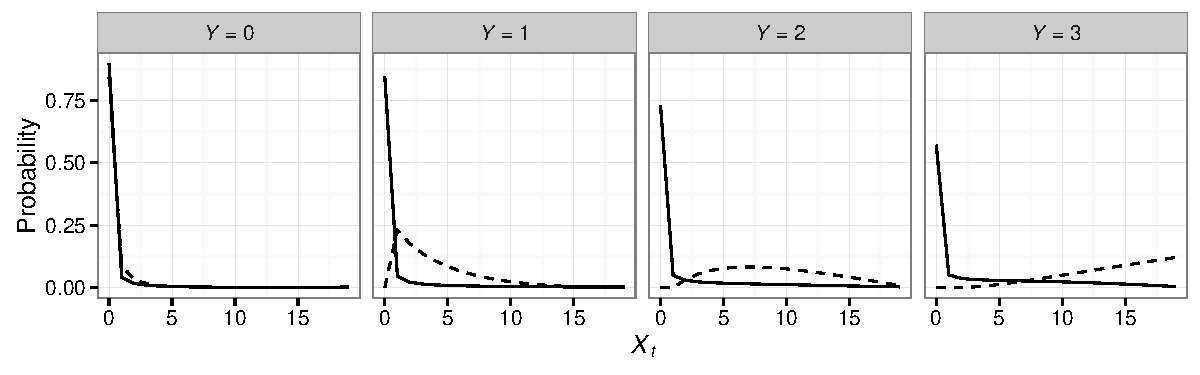
\includegraphics[width = 12cm]{cProb.pdf}
\caption{Conditional probabilities of allelic states in a site frequency spectrum of size $M=3$. The solid lines represent the conditional probabilities of an allelic state $y$ at $t=-s$, while the dashed lines represent the probabilities at $t=0$. The parameters were set to $\theta_a=0.05$, $\theta_c=0.1$, $s=200$ and $N=20$.}\label{cProb}
\end{figure}

\begin{figure}[ht]
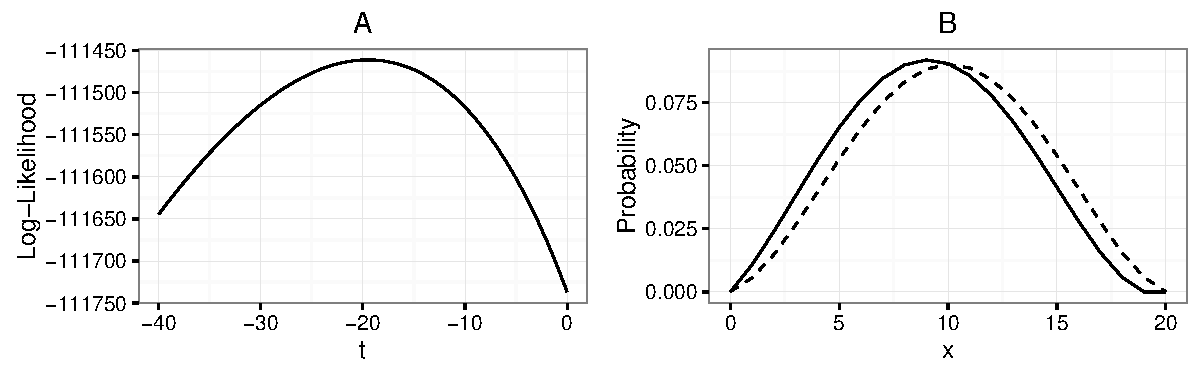
\includegraphics[width = 12cm]{twoPop_14_7_2016.pdf}
\caption{A) The log-likelihood of the split time $t$, given a joint SFS (Table~\ref{jointSFSdiscr}). B) The conditional probability for the allelic state with $y_1=1$ and $y_2=2$, at $t=-s$ (solid line) and $t=0$ (dashed line).}\label{twoPopdiscr}
\end{figure}

\begin{figure}[ht]
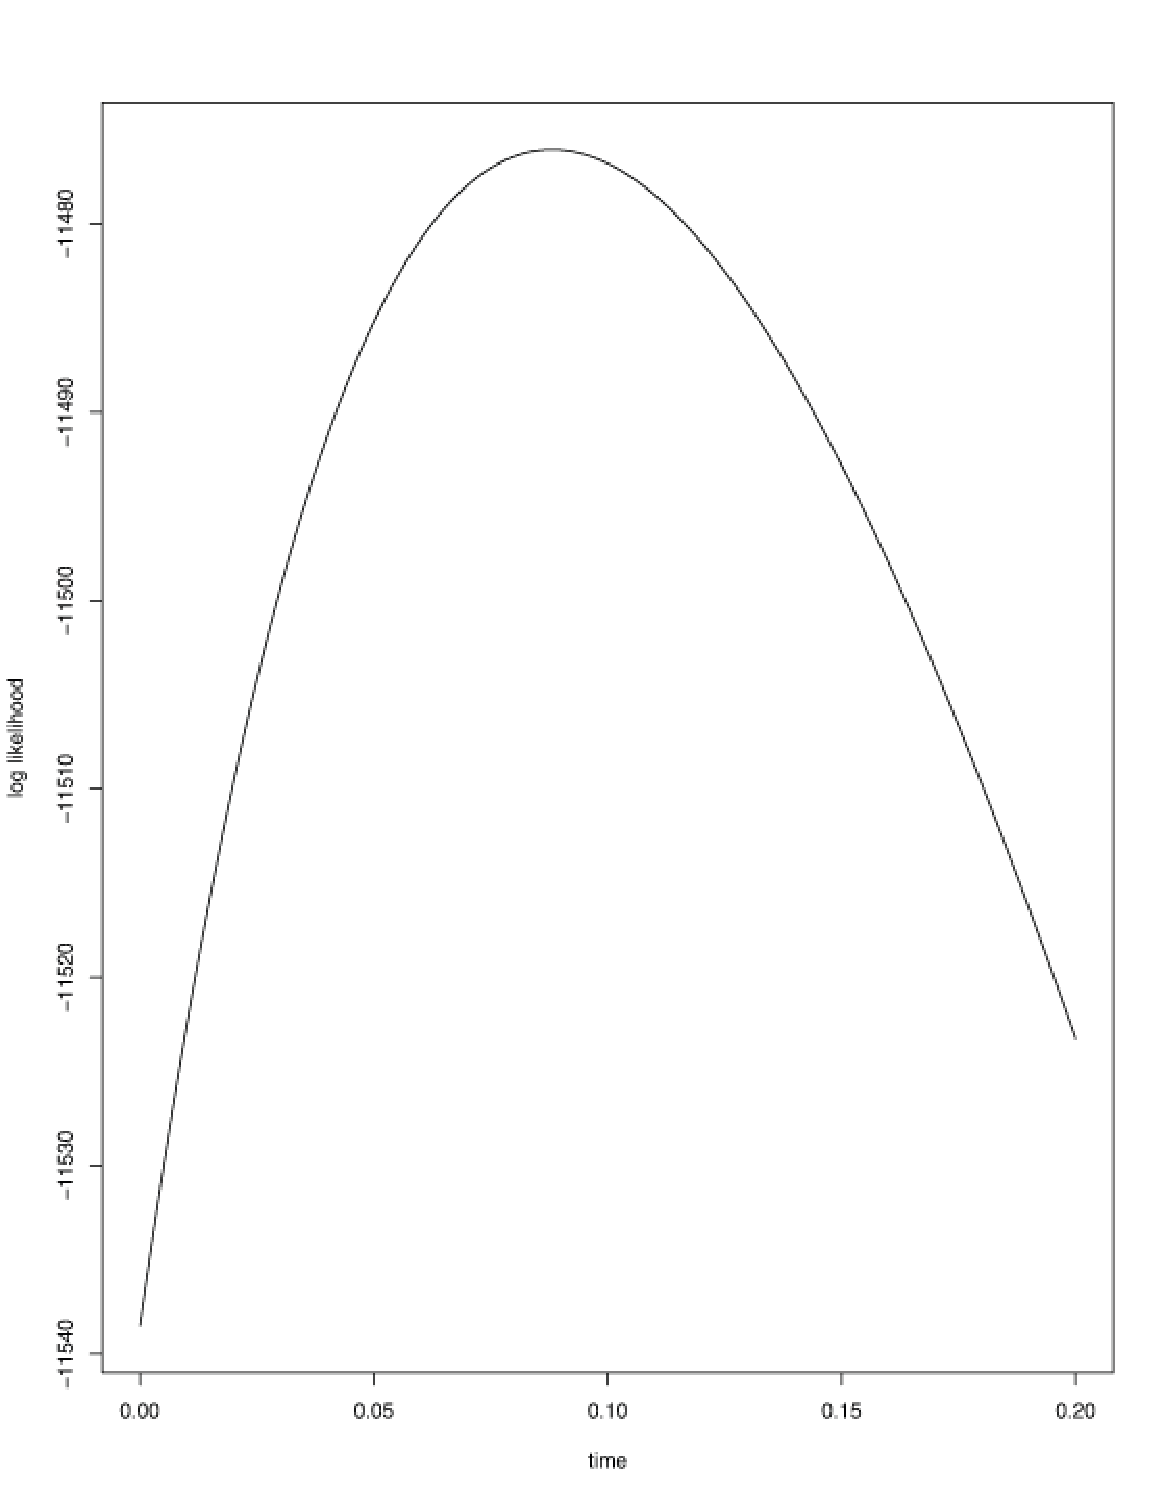
\includegraphics[width = 6cm]{forw_back_ll_cont.pdf}
\caption{The log-likelihood of the split time $\tau=0.1$, given a joint SFS (Table~\ref{jointSFScont}).}\label{twoPopcont}
\end{figure}

\newpage

\section*{Tables}

\begin{table}[ht]
\centering
%\fontsize{5}{5}\selectfont
\caption{A joint SFS simulated with a discrete Moran model with parameters $L=10^5$, $M_1=M_2=3$, $\alpha=2/3$, $\theta=0.1$, $s=20$ and $N=20$.}
  \begin{tabular}{lllll}
  \toprule
    $y$&$0$&$1$&$2$&$3$\\
    \midrule
    $0$  &$29185$ &$1244$ &$363$  &$83$\\       
    $1$  &$1247$  &$795$  &$576$  &$355$\\       
    $2$  &$376$   &$619$  &$798$  &$1317$\\      
    $3$  &$114$   &$347$  &$1286$ &$61295$\\    
    \bottomrule
  \end{tabular}\label{jointSFSdiscr}
\end{table}

\begin{table}[ht]
\centering
%\fontsize{5}{5}\selectfont
\caption{A joint SFS simulated with a continuous diffusion model with parameters $L=10^4$, $M_1=M_2=3$, $\alpha=2/3$, $\theta=0.1$, and $s=0.2$.}
  \begin{tabular}{lllll}
  \toprule
    $y$&$0$&$1$&$2$&$3$\\
    \midrule
    $0$  &$2915$ &$134$ &$36$  &$24$\\
    $1$  &$145$  &$50$ &$46$ &$53$\\
    $2$  &$40$   &$51$ &$69$ &$135$\\
    $3$  &$24$   &$50$  &$168$ &$6060$\\
    \bottomrule
  \end{tabular}\label{jointSFScont}
\end{table}




\end{document}

%%% Local Variables:
%%% mode: latex
%%% TeX-master: t
%%% End:
